\chapter{Theorie der linearen Antwort}
Dieses äusserst wichtige Thema behandelt die linearen passive Systeme, wie wir
sie aus der Elektrotechnik kennen. Hierbei bedeutet ``Passivität'', dass das
System im zeitlichen Mittel nur Arbeit bzw. Energie aufnimmt, wenn äussere
Kräfte darauf einwirken. Dieser Abschnitt folgt im wesentlichen der
Darstellung, wie sie in (Jaeckle, 1978) zu finden ist.
\section{Der gedämpfte harmonische Oszillator
\it Exkursion zur Drosophila melanogaster der Physik}\label{sec:gho}
Da der harmonische Oszillator in zahlreichen Variationen und auf den
verschiedensten Gebieten immer wieder anzutreffen ist, wollen wir ihm hier
einen extra Unterabschnitt widmen. 

Die Auslenkung $x(t)$ eines gedämpften harmonischen Oszillators als Antwort
auf eine von außen angelegte zeitabhängige Kraft $f(t)$ ist gegeben durch
die Differentialgleichung
\begin{equation}
  m\left(\frac{d^2}{dt^2}+\beta\frac{d}{dt}+\omega_0^2\right)x(t)=f(t)  
  \label{eq:gdho}
\end{equation}
wobei $\beta$ die Dämpfungskonstante bezeichne und $\omega_0/2\pi$ die
Eigenfrequenz des Oszillators ohne Dämpfung.

Für eine beliebige äussere Kraft $f(t)$ existiert eine sogenannte {\it
lineare Antwortfunktion} oder auch {\it Greensche Funktion} $G(\tau)$ genannt,
mit Hilfe derer wir die Lösung des Anfangswertproblems mit
$\lim_{t_0\rightarrow 0}x(t_0)=0$ und $\lim_{t_0\rightarrow 0}\dot{x}(t_0)=0$
auf folgende Weise schreiben können
\begin{equation}
  x(t)=\int_{-\infty}^{\infty}G(t-t')f(t')dt'
  \label{eq:solugreengdho}
\end{equation}
Die Greensche Funktion ist eine lineare Abbildung der Funktion $f(t)$ auf die
Funktion $x(t)$ (man zeige dass (\ref{eq:solugreengdho}) tatsächlich eine
lineare Abbildung ist!).

Für $\frac{\beta}{2}<\omega_0$, dem Fall schwacher Dämpfung, lautet die
Greensche Funktion 
\begin{equation}
  G(\tau)=\frac{1}{m\omega_r}e^{-\frac{\beta}{2}\tau}\sin(\omega_r\tau)\Theta(\tau)
  \label{eq:Greenfunction}
\end{equation}
wobei $\omega_r=\sqrt{\omega_0^2-\frac{\beta^2}{4}}$ die Resonanzfrequenz im
Dämpfungsfall bezeichne und 
\begin{equation*}
  \Theta(\tau)=\left\{\begin{array}{cc}1&\mbox{ für }\tau>0\\0&\mbox{ sonst. }\end{array}\right.
\end{equation*}
Diese Lösung des harmonischen Oszillators mit Hilfe einer linearen
Antwortfunktion oder der Greenschen Funktion kann in gleicher Weise auf eine
gro{\ss}e Klasse von Systemen linearer Differentialgleichungen verallgemeinert
werden.

Wir sehen im Fall des harmonischen Oszillators, dass die Greensche Funktion die
Differentialgleichung
\begin{equation}
  m\left(\frac{d^2}{d\tau^2}+\beta\frac{d}{d\tau}+\omega_0^2\right)G(\tau)=\delta(\tau)  
  \label{eq:dglGreensfunction}
\end{equation}
Dies zeigt man durch einsetzen von (\ref{eq:solugreengdho}) in (\ref{eq:gdho}).
Die Greensche Funktion beschreibt deshalb die Lösung der harmonischen
Oszillatorgleichung als Antwort auf einen Deltapuls, also die
Impulsantwortfunktion.
\begin{exercise}{Die Antwort des Oszillators}
Zeige mit Hilfe der Laplacetransformation, dass (\ref{eq:Greenfunction}) die
Impulsantwortfunktion des gedämpften harmonischen Oszillators ist.
\end{exercise}
Es interessiert uns besonders die harmonische Antwort des Oszillators.  Wir
suchen die Lösung von (\ref{eq:gdho}) bei einer Inhomogenität der Form
\begin{equation}\label{eq:harminh}
f(t)=\Re\{f_0\cdot e^{-izt}\}=|f_0| \cos(\omega t-\delta)e^{\eta t}\mbox{ mit }z=\omega
+i\eta\mbox{ und }\eta >0
\end{equation}
\begin{note}{Adiabatisches Einschalten}
$\eta >0$ entspricht einem langsamen ''adiabatischen'' Einschalten der externen
treibenden Kraft. Wir betrachten immer den Limes $\eta\rightarrow 0$
interessiert.
\end{note}
Wir suchen eine partikuläre Lösung der Form
\begin{equation}\label{eq:partsol}
x(t)=\Re\{x_0\cdot e^{-izt}\}=|x_0| \cos(\omega t-\delta-\phi)e^{\eta t}
\end{equation}
Wir setzen nun (\ref{eq:harminh}, \ref{eq:partsol}) in (\ref{eq:gdho}) ein und
erhalten damit für das Verhältnis der komplexen Amplituden
\begin{equation}\label{eq:dynsusz}
\frac{x_0}{f_0}=\frac{1/m}{-z^2-i\beta z+\omega_0^2}=\chi(z)
\end{equation}
Wir nennen $\chi(z)$ die {\it dynamische Suszeptibilität} des Systems, in unserem
Fall des harmonischen Oszillators. Die dynamische Suszeptibilät bestimmt die
Antwort $x(t)$ des gedämpften harmonischen Oszillators auf eine harmonische
treibende Kraft $f(t)$, die mit der Frequenz $\omega$ oszilliert. Wir können
die dynamische Suszeptibilität auch mit der Greenschen Funktion nach
(\ref{eq:solugreengdho}) erhalten. Der Vergleich der Ergebnisse zeigt, dass die
dynamische Suszeptibilität die Laplacetransformierte der Greenschen Funktion
ist
\begin{equation}\label{eq:suszept}
\chi(z) = \int_0^\infty G(t)e^{izt}dt
\end{equation}
\begin{note}{}
Zeige, dass die Form der Laplacetransformation in (\ref{eq:suszept}) äquivalent
derjenigen in (\ref{eq:Laplacetrafo}) ist!
\end{note}
Nun definieren wir uns den Fall der Resonanz und zwar auf zwei verschiedene
Arten. Einmal als die Frequenz, bei der der Oszillator mit der maximalen
Amplitude ''antwortet'' und zum anderen als diejenige, bei der seine
Leistungsaufnahme maximal ist. Für ersteres gilt
\begin{equation}\label{eq:ampres}
\lim_{\eta\rightarrow 0}|\chi(\omega +i\eta)|=
\frac{1}{m\sqrt{(\omega^2-\omega_0^2)^2+(\beta\omega)^2}}
\end{equation}
und das Maximum der Auslenkung liegt bei
$\omega_{max}=\sqrt{\omega_0^2-\beta^2/2}$, also etwas unterhalb der
natürlichen Frequenz $\omega_0$. Die momentane Leistungsaufnahme eines Systems,
die an ihm verrichtet wird, ist gegeben durch die äussere Kraft multipliziert
mit der zeitlichen Veränderung der Auslenkung - also der Geschwindigkeit - was
sich schreiben lässt als $P(t)=f(t)\cdot\dot{x}(t)$. Wir berechnen die über
eine Schwingungsperiode $T$ gemittelte Leistung als
\begin{equation}\label{eq:PMittel}
\overline{P(t)}=\frac{1}{T}\int_0^T f(t)\dot{x}(t)dt
\end{equation}
Um $\dot{x}(t)$ zu berechnen benutzen wir (\ref{eq:dynsusz}) und erhalten
zunächst 
\[x(t)=\Re [f_0\cdot\chi(z)\cdot e^{-izt}]\] 
Wir bilden die Ableitung und machen
den Gernzübergang $\eta\rightarrow 0$ und erhalten 
\begin{equation}\label{eq:xdot}
\dot{x}(t)=\omega\cdot |f_0|(-\chi'(\omega)\sin(\omega t)+\chi''(\omega)\cos(\omega t)
\end{equation}
Dabei haben wir folgenden Grenzübergang gemacht
\[ 
\lim_{\eta\rightarrow 0}\chi(\omega+i\eta)=\chi'(\omega)+i\chi''(\omega)
\]
Wenn wir dies in (\ref{eq:PMittel}) einsetzen, dann erhalten wir 
\begin{equation}\label{eq:PMittelChi}
\overline{P(t)}=\frac{1}{2}|f_0|^2\omega\chi''(\omega)
\end{equation}
Der wesentliche Faktor ist also
\begin{equation}\label{eq:PMittelFactor}
\omega\chi''(\omega)=\frac{\beta\omega^2/m}{(\omega^2-\omega_0^2)^2+\beta^2\omega^2}
\end{equation}
Die beiden Resonanzkurven für Amplituden- und Leistungsresonanz zeigen wir in
einem Diagramm in Bild \ref{fig:resonances}
\begin{figure}[!h]
\begin{center}
%\includegraphics[height=0.6\textwidth]{/Users/greiner/TeX/LectureNotes/Basics/SimulationMST/SIMOnlyD/Figures/resonanz.pdf}
\includegraphics[height=0.6\textwidth]{fig/resonanz.pdf}
\caption{Amplituden- und Leistungsresonanz eines gedämpften harmonischen Oszillators.\label{fig:resonances}}
\end{center}
\end{figure}\newpage
\begin{exercise}{Amplituden- und Leistungsresonanz}
Interpretiere die beiden Resonanzkurven aus Abbildung \ref{fig:resonances}!
\end{exercise}
%\begin{exercise}{Die Antworten des Relaxators}
%Gegeben die Differentialgleichung eines gedämpften harmonsichen Oszillators,
%wie wir sie in Abschnitt \ref{sec:gho} bereits kennen gelernt haben,
%\begin{equation}\label{eq:relaxator}
%\dot{x}(t)+\frac{1}{\tau} x(t)=f(t)
%\end{equation}
%\begin{enumerate}
%  \item Iterative Lösung: integrieren Sie (\ref{eq:relaxator}) für $f(t)=0$ und
%	$x(0)=x_0$ von $t=0$ bis $t$. Damit erhalten Sie
%	$x(t)=x_0+\int_0^t\left(-\frac{1}{\tau} x(\xi)\right)d\xi$. Wenden Sie nun den in Abschnitt
%	\ref{sec:analyticsolu} an und ermitteln Sie die Lösung.
%  \item Berechnen Sie die Antwortfunktionen für:
%	\begin{itemize}
%	  \item $f(t)=\delta(t)$ die 
%	  \item $f(t)=\Theta(t-t_0)$, wobei $\Theta(z)$ die Heavisidesche
%                Sprungfunktion darstellt, die $0$ ist für$z\le 0$ und $1$ sonst.
%	  \item $f(t)=\alpha t$, the famous "ramp response".
%	  \item $f(t)=\sin(\omega t)$, also die harmonische Antwort.
%	\end{itemize}
%  \item Das ganze mit Hilfe der Laplacetransformation. Geben Sie auch die
%	Lösung im Frequenzbereich an.
%\end{enumerate}
%%\input{Exercises/Chapter2/Relaxator.tex}
%\end{exercise}
%
\section{Die Funktion der linearen Antwort}
Im allgemeinen Fall eines linearen zeitinvarianten Systems (LTI-System) wissen
wir, dass die Antwortfunktion nur von der Zeitdifferenz $t-t'$ abhängt, d.h.
die allgemeine Antwort reduziert sich auf die Form wie beim harmonischen
Oszillator
\begin{equation}
  x(t)=\int_{-\infty}^{\infty}G_{LTI}(t,t')f(t')dt'=\int_{-\infty}^{\infty}G(t-t')f(t')dt'
  \label{eq:soluLTI}
\end{equation} 
Wir interessieren uns also nur für die Laplacetransformierte von $G(\tau)$,
wobei wir wissen, dass $G(\tau)=0$ für $\tau<0$. Dann ist die Antwort auf die
angelegte Kraft 
\begin{equation}
  x(t)=\int\limits_{-\infty}^{\infty}G(t-t')F(t')dt'
  \label{eq:Response}
\end{equation} 
$G(\tau)$ ist die reelle Systemfunktion. Wir nennen Sie die Funktion der
linearen Antwort. Das System solle sich kausal verhalten, was bedeutet, dass
$x(t)=0$ für alle Zeiten $t$, die vor dem Eischalten der Kraft $f(t)$ liegen.
Das bedeuet, dass $G(\tau)=0$ für $\tau<0$.

Ausserdem sollen $x(t)$ und $f(t)$ die momentane Arbeitsleistung des Systems
bestimmen durch 
\[P(t)=f(t)\cdot\dot{x}(t).\]
Passivität des Systems soll nun bedeuten, dass bei einer periodischen von
aussen anregenden Kraft, die mittlere von aussen geleistete Arbeit nicht
negativ ist.

Die Antwort auf eine periodische äußere Kraft
$f(t)=\Re\{f_0e^{-izt}\}$ mit $\Im\{z\}>0$ erhalten
wir aus (\ref{eq:Response}) zu $x(t)=\operatorname{Re}\{x_0e^{-izt}\}$, wobei
\[
  \frac{x_0}{f_0} = \chi(z) = \int_{-\infty}^\infty G(\tau)e^{iz\tau}d\tau 
\]
wie bereits in (\ref{eq:suszept}) gesehen. Das Integral ersteckt sich
weiterhin der Kausalität wegen nur auf positive Zeiten $\tau>0$. Wir schreiben
die Inverse Laplacetransformation der Suszeptibilität als
\begin{equation}
  G(\tau)=\frac{1}{2\pi}\int\limits_{-\infty+i\eta}^{+\infty+i\eta}e^{-iz\tau}\chi(z)dz=
  \frac{1}{2\pi}\int\limits_{-\infty}^{+\infty}e^{-i(\omega+i\eta)\tau}\chi(\omega+i\eta)d\omega,
  \quad \eta>0
  \label{eq:LinRespRueck}
\end{equation}
Den Beweis hierfür schauen wir uns im nächsten Abschnitt genauer an.

Zunächst benutzen wir die Zerlegung der Suszeptibilität nach Real- und
Imaginärteil, mit dem Grnzübergang, wie wir das schon im vorigen Abschnitt
getan haben
\[ 
\lim_{\eta\rightarrow 0}\chi(\omega+i\eta)=\chi'(\omega)+i\chi''(\omega)
\]
Dies erlaubt uns die Lösung $x(t)=\Re\{x_0e^{-izt}\}$ in zwei
verschiedenphasige Komponenten zu zerlegen
\begin{equation}
  x(t)=\Re\{x_0e^{-izt}\}=
  |f_0|e^{\eta t}\left(\chi'(\omega)\cos(\omega t-\varphi)
  +\chi''(\omega)sin(\omega t-\varphi)\right)
  \label{eq:Zweiphasig}
\end{equation}
Da $\chi(z)$ die Laplacetransformierte einer reellen Funktion ist, gilt
\[ [\chi(\omega+i\eta)]^*=[\chi(-\omega+i\eta)\]
Daraus wiederum folgt, dass der Realteil $\chi'$ eine gerade und der
Imaginärteil $\chi''$ eine ungerade Funktion von $\omega$ ist
\[ \chi'(-\omega)=\chi'(\omega),\quad \chi''(-\omega)=-\chi''(\omega) \]
Wir berechnen die mittlere Energieabsorption des Systems pro Zeiteinheit bei
einer periodischen Anregung mit einer äußeren Kraft der Frequenz
$\nu=\omega/2\pi$ und der Amplitude $f_0$:
\[
  \overline{P}=\frac{1}{T}\int_0^T f(t)\dot{x}(t)dt=
  \frac{1}{2}|f_0|^2\omega\chi''(\omega)
\]
Damit wird die Bedingung für die Passivität $\omega\chi''(\omega)\ge 0$.
%\section{Die Dispersionsrelationen}
%Mit Hilfe der Funktionentheorie läßt sich eine allgemeingültiger Zusammenhang
%herstellen. Es handelt sich hirbei um die \textit{Dispersionrelationen} oder
%auch \textit{Kramers-Kronig Relationen} genannt. Sie verknüpfen Real- und
%Imaginärteil der Suszeptibilität $\chi(\omega)$. Das bedeutet, dass das
%Verhalten eines linearen Systems durch eine einzige der Funktionen $G(\tau)$,
%$\chi'(\omega)$ oder $\chi''(\omega)$ vollständig bestimmt ist.
%
%Wir gehen von der dynamischen Suszeptibilität 
%\[ \chi(z) = \int_{-\infty}^\infty G(\tau)e^{iz\tau}d\tau \]
%aus. Der Integrationsbereich ist auf positive Zeiten $\tau$ beschränkt - wir
%erinnern uns, dass wir bei der Integration über $t'$ in (\ref{eq:Response})
%$t-t'=\tau$ gesetzt haben und die Funktion $G(t-t')$ nur für $t'<t$ von Null
%verschieden war, d.h. das System ist kausal - und der Expontentialfaktor drückt
%den Integranden für $\tau\rightarrow\infty$ gegen Null (wir haben $z=\omega
%+i\eta$). Damit ist 
%
